% Options for packages loaded elsewhere
\PassOptionsToPackage{unicode}{hyperref}
\PassOptionsToPackage{hyphens}{url}
\PassOptionsToPackage{dvipsnames,svgnames,x11names}{xcolor}
%
\documentclass[
  letterpaper,
  DIV=11,
  numbers=noendperiod]{scrartcl}

\usepackage{amsmath,amssymb}
\usepackage{lmodern}
\usepackage{iftex}
\ifPDFTeX
  \usepackage[T1]{fontenc}
  \usepackage[utf8]{inputenc}
  \usepackage{textcomp} % provide euro and other symbols
\else % if luatex or xetex
  \usepackage{unicode-math}
  \defaultfontfeatures{Scale=MatchLowercase}
  \defaultfontfeatures[\rmfamily]{Ligatures=TeX,Scale=1}
\fi
% Use upquote if available, for straight quotes in verbatim environments
\IfFileExists{upquote.sty}{\usepackage{upquote}}{}
\IfFileExists{microtype.sty}{% use microtype if available
  \usepackage[]{microtype}
  \UseMicrotypeSet[protrusion]{basicmath} % disable protrusion for tt fonts
}{}
\makeatletter
\@ifundefined{KOMAClassName}{% if non-KOMA class
  \IfFileExists{parskip.sty}{%
    \usepackage{parskip}
  }{% else
    \setlength{\parindent}{0pt}
    \setlength{\parskip}{6pt plus 2pt minus 1pt}}
}{% if KOMA class
  \KOMAoptions{parskip=half}}
\makeatother
\usepackage{xcolor}
\setlength{\emergencystretch}{3em} % prevent overfull lines
\setcounter{secnumdepth}{-\maxdimen} % remove section numbering
% Make \paragraph and \subparagraph free-standing
\ifx\paragraph\undefined\else
  \let\oldparagraph\paragraph
  \renewcommand{\paragraph}[1]{\oldparagraph{#1}\mbox{}}
\fi
\ifx\subparagraph\undefined\else
  \let\oldsubparagraph\subparagraph
  \renewcommand{\subparagraph}[1]{\oldsubparagraph{#1}\mbox{}}
\fi

\usepackage{color}
\usepackage{fancyvrb}
\newcommand{\VerbBar}{|}
\newcommand{\VERB}{\Verb[commandchars=\\\{\}]}
\DefineVerbatimEnvironment{Highlighting}{Verbatim}{commandchars=\\\{\}}
% Add ',fontsize=\small' for more characters per line
\usepackage{framed}
\definecolor{shadecolor}{RGB}{241,243,245}
\newenvironment{Shaded}{\begin{snugshade}}{\end{snugshade}}
\newcommand{\AlertTok}[1]{\textcolor[rgb]{0.68,0.00,0.00}{#1}}
\newcommand{\AnnotationTok}[1]{\textcolor[rgb]{0.37,0.37,0.37}{#1}}
\newcommand{\AttributeTok}[1]{\textcolor[rgb]{0.40,0.45,0.13}{#1}}
\newcommand{\BaseNTok}[1]{\textcolor[rgb]{0.68,0.00,0.00}{#1}}
\newcommand{\BuiltInTok}[1]{\textcolor[rgb]{0.00,0.23,0.31}{#1}}
\newcommand{\CharTok}[1]{\textcolor[rgb]{0.13,0.47,0.30}{#1}}
\newcommand{\CommentTok}[1]{\textcolor[rgb]{0.37,0.37,0.37}{#1}}
\newcommand{\CommentVarTok}[1]{\textcolor[rgb]{0.37,0.37,0.37}{\textit{#1}}}
\newcommand{\ConstantTok}[1]{\textcolor[rgb]{0.56,0.35,0.01}{#1}}
\newcommand{\ControlFlowTok}[1]{\textcolor[rgb]{0.00,0.23,0.31}{#1}}
\newcommand{\DataTypeTok}[1]{\textcolor[rgb]{0.68,0.00,0.00}{#1}}
\newcommand{\DecValTok}[1]{\textcolor[rgb]{0.68,0.00,0.00}{#1}}
\newcommand{\DocumentationTok}[1]{\textcolor[rgb]{0.37,0.37,0.37}{\textit{#1}}}
\newcommand{\ErrorTok}[1]{\textcolor[rgb]{0.68,0.00,0.00}{#1}}
\newcommand{\ExtensionTok}[1]{\textcolor[rgb]{0.00,0.23,0.31}{#1}}
\newcommand{\FloatTok}[1]{\textcolor[rgb]{0.68,0.00,0.00}{#1}}
\newcommand{\FunctionTok}[1]{\textcolor[rgb]{0.28,0.35,0.67}{#1}}
\newcommand{\ImportTok}[1]{\textcolor[rgb]{0.00,0.46,0.62}{#1}}
\newcommand{\InformationTok}[1]{\textcolor[rgb]{0.37,0.37,0.37}{#1}}
\newcommand{\KeywordTok}[1]{\textcolor[rgb]{0.00,0.23,0.31}{#1}}
\newcommand{\NormalTok}[1]{\textcolor[rgb]{0.00,0.23,0.31}{#1}}
\newcommand{\OperatorTok}[1]{\textcolor[rgb]{0.37,0.37,0.37}{#1}}
\newcommand{\OtherTok}[1]{\textcolor[rgb]{0.00,0.23,0.31}{#1}}
\newcommand{\PreprocessorTok}[1]{\textcolor[rgb]{0.68,0.00,0.00}{#1}}
\newcommand{\RegionMarkerTok}[1]{\textcolor[rgb]{0.00,0.23,0.31}{#1}}
\newcommand{\SpecialCharTok}[1]{\textcolor[rgb]{0.37,0.37,0.37}{#1}}
\newcommand{\SpecialStringTok}[1]{\textcolor[rgb]{0.13,0.47,0.30}{#1}}
\newcommand{\StringTok}[1]{\textcolor[rgb]{0.13,0.47,0.30}{#1}}
\newcommand{\VariableTok}[1]{\textcolor[rgb]{0.07,0.07,0.07}{#1}}
\newcommand{\VerbatimStringTok}[1]{\textcolor[rgb]{0.13,0.47,0.30}{#1}}
\newcommand{\WarningTok}[1]{\textcolor[rgb]{0.37,0.37,0.37}{\textit{#1}}}

\providecommand{\tightlist}{%
  \setlength{\itemsep}{0pt}\setlength{\parskip}{0pt}}\usepackage{longtable,booktabs,array}
\usepackage{calc} % for calculating minipage widths
% Correct order of tables after \paragraph or \subparagraph
\usepackage{etoolbox}
\makeatletter
\patchcmd\longtable{\par}{\if@noskipsec\mbox{}\fi\par}{}{}
\makeatother
% Allow footnotes in longtable head/foot
\IfFileExists{footnotehyper.sty}{\usepackage{footnotehyper}}{\usepackage{footnote}}
\makesavenoteenv{longtable}
\usepackage{graphicx}
\makeatletter
\def\maxwidth{\ifdim\Gin@nat@width>\linewidth\linewidth\else\Gin@nat@width\fi}
\def\maxheight{\ifdim\Gin@nat@height>\textheight\textheight\else\Gin@nat@height\fi}
\makeatother
% Scale images if necessary, so that they will not overflow the page
% margins by default, and it is still possible to overwrite the defaults
% using explicit options in \includegraphics[width, height, ...]{}
\setkeys{Gin}{width=\maxwidth,height=\maxheight,keepaspectratio}
% Set default figure placement to htbp
\makeatletter
\def\fps@figure{htbp}
\makeatother

\KOMAoption{captions}{tableheading}
\makeatletter
\@ifpackageloaded{tcolorbox}{}{\usepackage[many]{tcolorbox}}
\@ifpackageloaded{fontawesome5}{}{\usepackage{fontawesome5}}
\definecolor{quarto-callout-color}{HTML}{909090}
\definecolor{quarto-callout-note-color}{HTML}{0758E5}
\definecolor{quarto-callout-important-color}{HTML}{CC1914}
\definecolor{quarto-callout-warning-color}{HTML}{EB9113}
\definecolor{quarto-callout-tip-color}{HTML}{00A047}
\definecolor{quarto-callout-caution-color}{HTML}{FC5300}
\definecolor{quarto-callout-color-frame}{HTML}{acacac}
\definecolor{quarto-callout-note-color-frame}{HTML}{4582ec}
\definecolor{quarto-callout-important-color-frame}{HTML}{d9534f}
\definecolor{quarto-callout-warning-color-frame}{HTML}{f0ad4e}
\definecolor{quarto-callout-tip-color-frame}{HTML}{02b875}
\definecolor{quarto-callout-caution-color-frame}{HTML}{fd7e14}
\makeatother
\makeatletter
\makeatother
\makeatletter
\makeatother
\makeatletter
\@ifpackageloaded{caption}{}{\usepackage{caption}}
\AtBeginDocument{%
\ifdefined\contentsname
  \renewcommand*\contentsname{Table of contents}
\else
  \newcommand\contentsname{Table of contents}
\fi
\ifdefined\listfigurename
  \renewcommand*\listfigurename{List of Figures}
\else
  \newcommand\listfigurename{List of Figures}
\fi
\ifdefined\listtablename
  \renewcommand*\listtablename{List of Tables}
\else
  \newcommand\listtablename{List of Tables}
\fi
\ifdefined\figurename
  \renewcommand*\figurename{Figure}
\else
  \newcommand\figurename{Figure}
\fi
\ifdefined\tablename
  \renewcommand*\tablename{Table}
\else
  \newcommand\tablename{Table}
\fi
}
\@ifpackageloaded{float}{}{\usepackage{float}}
\floatstyle{ruled}
\@ifundefined{c@chapter}{\newfloat{codelisting}{h}{lop}}{\newfloat{codelisting}{h}{lop}[chapter]}
\floatname{codelisting}{Listing}
\newcommand*\listoflistings{\listof{codelisting}{List of Listings}}
\makeatother
\makeatletter
\@ifpackageloaded{caption}{}{\usepackage{caption}}
\@ifpackageloaded{subcaption}{}{\usepackage{subcaption}}
\makeatother
\makeatletter
\@ifpackageloaded{tcolorbox}{}{\usepackage[many]{tcolorbox}}
\makeatother
\makeatletter
\@ifundefined{shadecolor}{\definecolor{shadecolor}{rgb}{.97, .97, .97}}
\makeatother
\makeatletter
\makeatother
\ifLuaTeX
  \usepackage{selnolig}  % disable illegal ligatures
\fi
\IfFileExists{bookmark.sty}{\usepackage{bookmark}}{\usepackage{hyperref}}
\IfFileExists{xurl.sty}{\usepackage{xurl}}{} % add URL line breaks if available
\urlstyle{same} % disable monospaced font for URLs
\hypersetup{
  pdftitle={Álgebra Linear Computacional},
  pdfauthor={Heitor S. Ramos   ramosh@dcc.ufmg.br},
  colorlinks=true,
  linkcolor={blue},
  filecolor={Maroon},
  citecolor={Blue},
  urlcolor={Blue},
  pdfcreator={LaTeX via pandoc}}

\title{Álgebra Linear Computacional}
\usepackage{etoolbox}
\makeatletter
\providecommand{\subtitle}[1]{% add subtitle to \maketitle
  \apptocmd{\@title}{\par {\large #1 \par}}{}{}
}
\makeatother
\subtitle{Aula 04: Autovalores e Autovetores}
\author{Heitor S. Ramos ramosh@dcc.ufmg.br}
\date{}

\begin{document}
\maketitle
\ifdefined\Shaded\renewenvironment{Shaded}{\begin{tcolorbox}[frame hidden, enhanced, breakable, borderline west={3pt}{0pt}{shadecolor}, interior hidden, boxrule=0pt, sharp corners]}{\end{tcolorbox}}\fi

\hypertarget{cruxe9ditos}{%
\subsection{Créditos}\label{cruxe9ditos}}

\begin{tcolorbox}[enhanced jigsaw, arc=.35mm, opacityback=0, bottomtitle=1mm, left=2mm, coltitle=black, rightrule=.15mm, colbacktitle=quarto-callout-important-color!10!white, breakable, opacitybacktitle=0.6, bottomrule=.15mm, title=\textcolor{quarto-callout-important-color}{\faExclamation}\hspace{0.5em}{Important}, titlerule=0mm, colframe=quarto-callout-important-color-frame, toprule=.15mm, toptitle=1mm, leftrule=.75mm, colback=white]
Os slides desse curso são fortemente baseados no curso do Fabrício Murai
e do Erickson Nascimento
\end{tcolorbox}

\hypertarget{objetivos-de-aprendizagem}{%
\subsection{Objetivos de Aprendizagem}\label{objetivos-de-aprendizagem}}

\begin{itemize}
\tightlist
\item
  Saber calcular autov* de matrizes \(2\times 2\) manualmente
\item
  Saber escrever polinômio característico para matrizes grandes e saber
  que suas raízes são os autovalores
\item
  Conhecer relação entre traço, determinante e autovalores
\item
  Conhecer relação entre autov* de \(A\), de \(A^k\), de \(A^{-1}\), e
  de \(A+sI\)
\item
  Saber definir matrizes similares e conhecer relação entre seus autov*
\item
  Saber que, quando existe, a decomposição espectral \(A=XΛ\) permite
  diagonalizar uma matriz
\item
  Saber calcular \(A^k\) e \(A^kv\) dada a decomposição \(A=XΛ\)
\end{itemize}

\hypertarget{referuxeancias}{%
\subsection{Referências}\label{referuxeancias}}

\begin{itemize}
\tightlist
\item
  \href{https://en.wikipedia.org/wiki/Eigendecomposition_of_a_matrix}{Wikipedia}
\item
  \href{https://youtu.be/PFDu9oVAE-g}{3blue1brown}
\item
  \href{http://www.ime.unicamp.br/~andreani/matrizes/capitulo7.pdf}{Matrix
  Analysis, Chapter 7 (Carl Mayer)}
\end{itemize}

\hypertarget{multiplicauxe7uxe3o-entre-matrix-e-vetor}{%
\subsection{Multiplicação entre matrix e
vetor}\label{multiplicauxe7uxe3o-entre-matrix-e-vetor}}

\[ \begin{bmatrix}2 & 1\\ 1 & 2\end{bmatrix}\begin{bmatrix}2\\3\end{bmatrix}=\begin{bmatrix}7\\8\end{bmatrix}\]

\[ 2\begin{bmatrix}2 \\ 1\end{bmatrix} + 3\begin{bmatrix}1 \\ 2\end{bmatrix}=\begin{bmatrix}7\\8\end{bmatrix}\]

\begin{Shaded}
\begin{Highlighting}[]
\ImportTok{import}\NormalTok{ matplotlib.pyplot }\ImportTok{as}\NormalTok{ plt}
\ImportTok{import}\NormalTok{ numpy }\ImportTok{as}\NormalTok{ np}
\NormalTok{V }\OperatorTok{=}\NormalTok{ np.array([[}\DecValTok{4}\NormalTok{,}\DecValTok{2}\NormalTok{], [}\DecValTok{3}\NormalTok{,}\DecValTok{6}\NormalTok{], [}\DecValTok{7}\NormalTok{,}\DecValTok{8}\NormalTok{],[}\DecValTok{2}\NormalTok{,}\DecValTok{1}\NormalTok{], [}\DecValTok{1}\NormalTok{,}\DecValTok{2}\NormalTok{],[}\DecValTok{4}\NormalTok{,}\DecValTok{2}\NormalTok{],[}\DecValTok{3}\NormalTok{,}\DecValTok{6}\NormalTok{],[}\DecValTok{2}\NormalTok{,}\DecValTok{3}\NormalTok{]])}
\NormalTok{origin }\OperatorTok{=}\NormalTok{ ([}\DecValTok{0}\NormalTok{,}\DecValTok{0}\NormalTok{,}\DecValTok{0}\NormalTok{,}\DecValTok{0}\NormalTok{,}\DecValTok{0}\NormalTok{,}\DecValTok{3}\NormalTok{,}\DecValTok{4}\NormalTok{,}\DecValTok{0}\NormalTok{],[}\DecValTok{0}\NormalTok{,}\DecValTok{0}\NormalTok{,}\DecValTok{0}\NormalTok{,}\DecValTok{0}\NormalTok{,}\DecValTok{0}\NormalTok{,}\DecValTok{6}\NormalTok{,}\DecValTok{2}\NormalTok{,}\DecValTok{0}\NormalTok{])}
\NormalTok{fig }\OperatorTok{=}\NormalTok{ plt.figure()}
\NormalTok{plt.quiver(}\OperatorTok{*}\NormalTok{origin, V[:,}\DecValTok{0}\NormalTok{], V[:,}\DecValTok{1}\NormalTok{], angles}\OperatorTok{=}\StringTok{\textquotesingle{}xy\textquotesingle{}}\NormalTok{, scale\_units}\OperatorTok{=}\StringTok{\textquotesingle{}xy\textquotesingle{}}\NormalTok{, scale}\OperatorTok{=}\DecValTok{1}\NormalTok{, color}\OperatorTok{=}\NormalTok{[}\StringTok{\textquotesingle{}red\textquotesingle{}}\NormalTok{, }\StringTok{\textquotesingle{}red\textquotesingle{}}\NormalTok{, }\StringTok{\textquotesingle{}green\textquotesingle{}}\NormalTok{, }\StringTok{\textquotesingle{}gray\textquotesingle{}}\NormalTok{,}\StringTok{\textquotesingle{}gray\textquotesingle{}}\NormalTok{,}\StringTok{\textquotesingle{}blue\textquotesingle{}}\NormalTok{,}\StringTok{\textquotesingle{}blue\textquotesingle{}}\NormalTok{,}\StringTok{\textquotesingle{}yellow\textquotesingle{}}\NormalTok{])}
\NormalTok{plt.xlim((}\DecValTok{0}\NormalTok{,}\DecValTok{10}\NormalTok{))}
\NormalTok{plt.ylim((}\DecValTok{0}\NormalTok{,}\DecValTok{10}\NormalTok{)) }
\NormalTok{plt.draw()}
\NormalTok{plt.show()}
\end{Highlighting}
\end{Shaded}

\begin{figure}[H]

{\centering 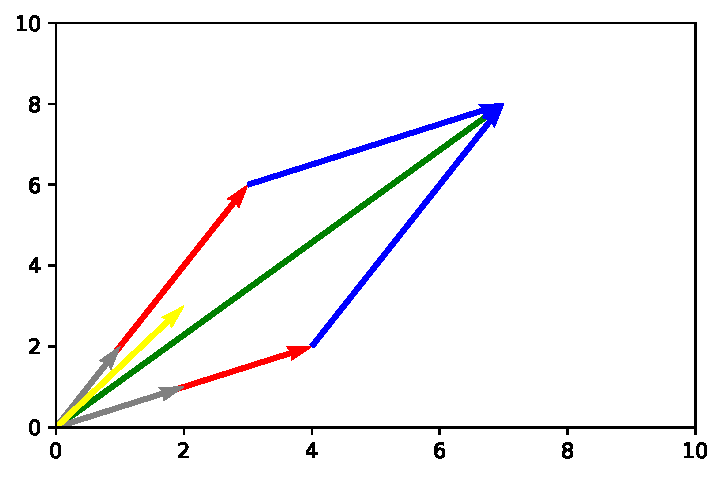
\includegraphics{Aula04_files/figure-pdf/fig1-output-1.pdf}

}

\caption{Produto Matrix x Vetor}

\end{figure}

\hypertarget{multiplicauxe7uxe3o-entre-matrix-e-vetor-1}{%
\subsection{Multiplicação entre matrix e
vetor}\label{multiplicauxe7uxe3o-entre-matrix-e-vetor-1}}

\[ \begin{bmatrix}2 & 1\\ 1 & 2\end{bmatrix}\begin{bmatrix}1\\1\end{bmatrix}=\begin{bmatrix}3\\3\end{bmatrix}\]

\[ 1\begin{bmatrix}2 \\ 1\end{bmatrix} + 1\begin{bmatrix}1 \\ 2\end{bmatrix}=3\begin{bmatrix}1\\1\end{bmatrix}\]

\begin{Shaded}
\begin{Highlighting}[]
\ImportTok{import}\NormalTok{ matplotlib.pyplot }\ImportTok{as}\NormalTok{ plt}
\ImportTok{import}\NormalTok{ numpy }\ImportTok{as}\NormalTok{ np}
\NormalTok{V }\OperatorTok{=}\NormalTok{ np.array([[}\DecValTok{1}\NormalTok{,}\DecValTok{2}\NormalTok{], [}\DecValTok{2}\NormalTok{,}\DecValTok{1}\NormalTok{], [}\DecValTok{3}\NormalTok{,}\DecValTok{3}\NormalTok{],[}\DecValTok{2}\NormalTok{,}\DecValTok{1}\NormalTok{],[}\DecValTok{1}\NormalTok{,}\DecValTok{2}\NormalTok{],[}\DecValTok{1}\NormalTok{,}\DecValTok{1}\NormalTok{]])}
\NormalTok{origin }\OperatorTok{=}\NormalTok{ ([}\DecValTok{0}\NormalTok{,}\DecValTok{0}\NormalTok{,}\DecValTok{0}\NormalTok{,}\DecValTok{1}\NormalTok{,}\DecValTok{2}\NormalTok{,}\DecValTok{0}\NormalTok{],[}\DecValTok{0}\NormalTok{,}\DecValTok{0}\NormalTok{,}\DecValTok{0}\NormalTok{,}\DecValTok{2}\NormalTok{,}\DecValTok{1}\NormalTok{,}\DecValTok{0}\NormalTok{])}
\NormalTok{fig }\OperatorTok{=}\NormalTok{ plt.figure()}
\NormalTok{plt.quiver(}\OperatorTok{*}\NormalTok{origin, V[:,}\DecValTok{0}\NormalTok{], V[:,}\DecValTok{1}\NormalTok{], angles}\OperatorTok{=}\StringTok{\textquotesingle{}xy\textquotesingle{}}\NormalTok{, scale\_units}\OperatorTok{=}\StringTok{\textquotesingle{}xy\textquotesingle{}}\NormalTok{, scale}\OperatorTok{=}\DecValTok{1}\NormalTok{, color}\OperatorTok{=}\NormalTok{[}\StringTok{\textquotesingle{}red\textquotesingle{}}\NormalTok{, }\StringTok{\textquotesingle{}red\textquotesingle{}}\NormalTok{, }\StringTok{\textquotesingle{}green\textquotesingle{}}\NormalTok{,}\StringTok{\textquotesingle{}blue\textquotesingle{}}\NormalTok{,}\StringTok{\textquotesingle{}blue\textquotesingle{}}\NormalTok{,}\StringTok{\textquotesingle{}yellow\textquotesingle{}}\NormalTok{])}
\NormalTok{plt.xlim((}\DecValTok{0}\NormalTok{,}\DecValTok{4}\NormalTok{))}
\NormalTok{plt.ylim((}\DecValTok{0}\NormalTok{,}\DecValTok{4}\NormalTok{)) }
\NormalTok{plt.draw()}
\NormalTok{plt.show()}
\end{Highlighting}
\end{Shaded}

\begin{figure}[H]

{\centering 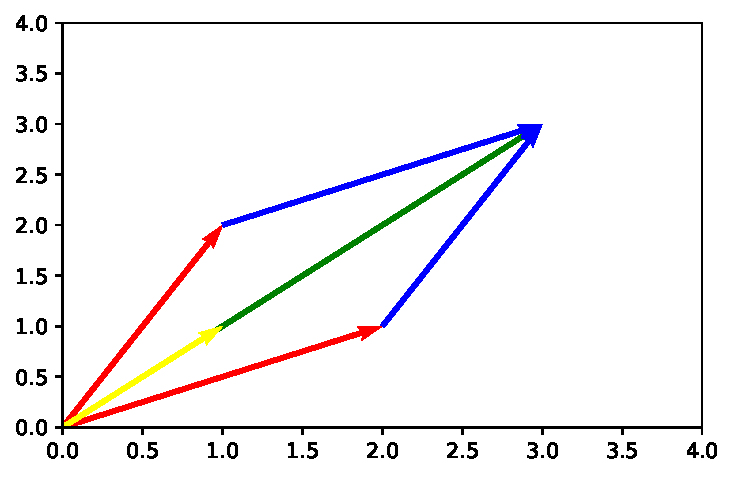
\includegraphics{Aula04_files/figure-pdf/fig2-output-1.pdf}

}

\caption{Produto Matrix x Vetor}

\end{figure}

\begin{tcolorbox}[enhanced jigsaw, arc=.35mm, opacityback=0, bottomtitle=1mm, left=2mm, coltitle=black, rightrule=.15mm, colbacktitle=quarto-callout-note-color!10!white, breakable, opacitybacktitle=0.6, bottomrule=.15mm, title=\textcolor{quarto-callout-note-color}{\faInfo}\hspace{0.5em}{Note}, titlerule=0mm, colframe=quarto-callout-note-color-frame, toprule=.15mm, toptitle=1mm, leftrule=.75mm, colback=white]
Observe que nesse caso temos que \(Av = \lambda v\)
\end{tcolorbox}

\hypertarget{autovalor-e-autovetor}{%
\subsection{Autovalor e Autovetor}\label{autovalor-e-autovetor}}

\begin{itemize}
\tightlist
\item
  Seja \(A\) uma matriz quadrada \(m\times m\)
\end{itemize}

\[Ax = \lambda x\]

\begin{tcolorbox}[enhanced jigsaw, arc=.35mm, opacityback=0, bottomtitle=1mm, left=2mm, coltitle=black, rightrule=.15mm, colbacktitle=quarto-callout-note-color!10!white, breakable, opacitybacktitle=0.6, bottomrule=.15mm, title=\textcolor{quarto-callout-note-color}{\faInfo}\hspace{0.5em}{Equação Característica}, titlerule=0mm, colframe=quarto-callout-note-color-frame, toprule=.15mm, toptitle=1mm, leftrule=.75mm, colback=white]
\[\begin{align}Ax -\lambda x &= 0\\
Ax -\lambda Ix &= 0\\
(A -\lambda I)x &= 0\\
det(M) &= 0, M = A- \lambda x\\
det((A - \lambda I)) &= 0 \rightarrow \text{Polinômio de grau } m \text{ em } \lambda \end{align}\]
\end{tcolorbox}

\hypertarget{calculando-autovalores-e-autovetores}{%
\subsection{Calculando Autovalores e
Autovetores}\label{calculando-autovalores-e-autovetores}}

\[ S = \begin{bmatrix}2 & 1\\ 1 & 2\end{bmatrix}\]

\begin{tcolorbox}[enhanced jigsaw, arc=.35mm, opacityback=0, bottomtitle=1mm, left=2mm, coltitle=black, rightrule=.15mm, colbacktitle=quarto-callout-note-color!10!white, breakable, opacitybacktitle=0.6, bottomrule=.15mm, title=\textcolor{quarto-callout-note-color}{\faInfo}\hspace{0.5em}{Polinômio Característico}, titlerule=0mm, colframe=quarto-callout-note-color-frame, toprule=.15mm, toptitle=1mm, leftrule=.75mm, colback=white]

\begin{itemize}
\tightlist
\item
  Cálculo dos autovalores
\end{itemize}

\[M = S - \lambda I \\ M =\begin{bmatrix}2-\lambda & 1 \\ 1 & 2-\lambda\end{bmatrix} \\ det(M) = 0 \\ (2- \lambda)^2 -1 =0 \\ 4 - 4\lambda + \lambda^2 -1 =0 \\ \lambda^2 - 4 \lambda + 3=0 \\ \begin{cases} \lambda_1 =1 \\ \lambda_2 =3 \end{cases} \]

\begin{itemize}
\tightlist
\item
  Cálculo dos autovetores \begin{align}
  Sx &= \lambda_1x & Sy &= \lambda_2 y\\
  (S-\lambda_1 I)x &=0 & (S-\lambda_2 I)y &=0\\
  \begin{bmatrix}1 & 1 \\ 1 & 1\end{bmatrix}x &=0 & \begin{bmatrix}-1 & 1 \\ 1 & -1\end{bmatrix}y &=0 \\
  x_1\begin{bmatrix}1 \\ 1\end{bmatrix} + x_2\begin{bmatrix}1 \\ 1\end{bmatrix} &= 0 & y_1\begin{bmatrix}-1 \\ 1\end{bmatrix} + y_2\begin{bmatrix}1 \\ -1\end{bmatrix} &= 0\\
  x &= \begin{bmatrix} 1\\-1\end{bmatrix} & y &= \begin{bmatrix} 1\\1\end{bmatrix}
  \end{align}
\end{itemize}

\end{tcolorbox}

\hypertarget{trauxe7o-determinante-e-autovalores}{%
\subsection{Traço, Determinante e
Autovalores}\label{trauxe7o-determinante-e-autovalores}}

\begin{itemize}
\item
  Traço: Soma da diagonal da matriz - igual à soma dos autovalores

  \[ \text{trace}(A) = \text{tr}(A) = \sum_{i=1}^m \lambda_i\]
\item
  Determinante: Produto dos autovalores
\end{itemize}

\[ det(A) = \mid A \mid = \prod_{i=1}^m \lambda_i\]

\hypertarget{autovalores-complexos}{%
\subsection{Autovalores Complexos}\label{autovalores-complexos}}

\[ R(\pi/2) = \begin{bmatrix}\cos(\pi/2)& -\sin(\pi/2)\\ \sin(\pi/2) & \cos(\pi/2)\end{bmatrix} = \begin{bmatrix}0 & -1 \\ 1 & 0\end{bmatrix}\]

\usepackage{gensymb}

\begin{itemize}
\tightlist
\item
  matriz que rotaciona \(90^\text{o}\) um vetor qualquer
\item
  claramente não tem autovalores reais (por quê?)
\end{itemize}

\[ det \left( \begin{bmatrix}-\lambda&-1\\1&-\lambda\end{bmatrix} \right) = 0 \\ \lambda^2 + 1 =0 \\ \lambda^2 = -1 \\ \begin{cases}\lambda = i\\ \lambda = -i\end{cases}\]

\hypertarget{potuxeancia-da-matriz-a}{%
\subsection{Potência da matriz A}\label{potuxeancia-da-matriz-a}}

\begin{itemize}
\tightlist
\item
  \(x\) é autovetor de \(A \Leftrightarrow x\) é autovetor da matriz
  \(B = A^2\)
\end{itemize}

\begin{tcolorbox}[enhanced jigsaw, arc=.35mm, opacityback=0, bottomtitle=1mm, left=2mm, coltitle=black, rightrule=.15mm, colbacktitle=quarto-callout-note-color!10!white, breakable, opacitybacktitle=0.6, bottomrule=.15mm, title=\textcolor{quarto-callout-note-color}{\faInfo}\hspace{0.5em}{Prova}, titlerule=0mm, colframe=quarto-callout-note-color-frame, toprule=.15mm, toptitle=1mm, leftrule=.75mm, colback=white]
\begin{equation}
Ax = \lambda x \Rightarrow A(Ax) = A(\lambda y)\\
A^2x = \lambda Ax\\
A^2x = \lambda (\lambda x)\\
A^2x = \lambda^2 x
\end{equation}
\end{tcolorbox}

\[ A^kx = \lambda^k x\]

\hypertarget{matriz-inversa-e-autovalor}{%
\subsection{Matriz inversa e
autovalor}\label{matriz-inversa-e-autovalor}}

\[A^{-1}x = \frac{1}{\lambda}x\]

\begin{tcolorbox}[enhanced jigsaw, arc=.35mm, opacityback=0, bottomtitle=1mm, left=2mm, coltitle=black, rightrule=.15mm, colbacktitle=quarto-callout-note-color!10!white, breakable, opacitybacktitle=0.6, bottomrule=.15mm, title=\textcolor{quarto-callout-note-color}{\faInfo}\hspace{0.5em}{Prova}, titlerule=0mm, colframe=quarto-callout-note-color-frame, toprule=.15mm, toptitle=1mm, leftrule=.75mm, colback=white]
\begin{equation}
Ax = \lambda x\\
A^{-1}Ax = \lambda A^{-1}x\\
Ix = \lambda A^{-1}x\\ 
A^{-1}x = \frac{1}{\lambda}x
\end{equation}
\end{tcolorbox}

\hypertarget{o-que-acontece-com-os-autovalores-e-autovetores-de-a-se-a-for-deslocada-para-a-a-si}{%
\subsection{\texorpdfstring{O que acontece com os autovalores e
autovetores de \(A\) se \(A\) for deslocada para
\(A = A + sI\)?}{O que acontece com os autovalores e autovetores de A se A for deslocada para A = A + sI?}}\label{o-que-acontece-com-os-autovalores-e-autovetores-de-a-se-a-for-deslocada-para-a-a-si}}

\[ Ax = \lambda x\]

\begin{enumerate}
\def\labelenumi{\arabic{enumi}.}
\item
  Autovalores

  \begin{itemize}
  \tightlist
  \item
    considere \(\lambda'\) os autovalores de \(A+ sI\)
  \item
    considere \(y\) autovetor de \(A + sI\) \begin{equation}
    (A+ sI)x = Ax + sx\\ 
    (A+sI)x= \lambda x + sx\\ 
    (A+sI)x = (\lambda + s)x\\
    \text{observe que } \lambda+s = \lambda'\\
    \end{equation}
  \end{itemize}
\item
  Autovetores \begin{equation}
  (A + sI)y = \lambda'y\\ 
  (A + sI - \lambda'I)y = 0\\ 
  (A - (\lambda' -s)I)y = 0\\
  \text{observe que } \lambda'-s = \lambda\\
  (A - \lambda I)y = 0
  \end{equation}
\end{enumerate}

\hypertarget{autovetores-e-a-matriz-a}{%
\subsection{\texorpdfstring{Autovetores e a matriz
\(A\)}{Autovetores e a matriz A}}\label{autovetores-e-a-matriz-a}}

\begin{itemize}
\item
  Muitas matrizes \(n\times n\) possuem \(n\) autovetores independentes

  \begin{itemize}
  \tightlist
  \item
    nesse caso, um vetor \(v\) \(n\)-dimensional pode ser escrito como
    uma combinação dos autovetores
  \end{itemize}

  \[ v = c_1x_1+\ldots + c_nx_n\]

  \[ Av = c_1\lambda_1x_1+\ldots + c_n\lambda_nx_n\]
\end{itemize}

\begin{tcolorbox}[enhanced jigsaw, arc=.35mm, opacityback=0, bottomtitle=1mm, left=2mm, coltitle=black, rightrule=.15mm, colbacktitle=quarto-callout-note-color!10!white, breakable, opacitybacktitle=0.6, bottomrule=.15mm, title=\textcolor{quarto-callout-note-color}{\faInfo}\hspace{0.5em}{Note}, titlerule=0mm, colframe=quarto-callout-note-color-frame, toprule=.15mm, toptitle=1mm, leftrule=.75mm, colback=white]
\[ Av = A(c_1x_1 + c_2x_2 + \ldots + c_nx_n)\\ Av = c_1Ax_1 + c_2Ax_2 + \ldots + c_nAx_n\\ Av = c_1\lambda_1x_1 + c_2\lambda_2x_2 + \ldots + c_n\lambda_nx_n\]

\[ A^2v = A(c_1\lambda_1x_1 + c_2\lambda_2x_2 + \ldots + c_n\lambda_nx_n)\\ A^2v = c_1\lambda_1Ax_1 + c_2\lambda_2Ax_2 + \ldots + c_n\lambda_nAx_n\\ A^2v = c_1\lambda_1^2x_1 + c_2\lambda_2^2x_2 + \ldots + c_n\lambda_n^2x_n\]
\end{tcolorbox}

\hypertarget{autovetores-e-a-matriz-a-1}{%
\subsection{\texorpdfstring{Autovetores e a matriz
\(A\)}{Autovetores e a matriz A}}\label{autovetores-e-a-matriz-a-1}}

\[ A^kv = c_1\lambda_1^kx_1 + \ldots + c_n\lambda_n^kx_n\]

\begin{itemize}
\tightlist
\item
  suponha que os autovalores ordenados apareçam da seguinte maneira
\end{itemize}

\[ \mid \lambda_1 \mid, \ldots, \mid \lambda_j\mid, \ldots, \mid \lambda_n\mid\]

\begin{itemize}
\tightlist
\item
  suponha também que \(\mid \lambda_j \mid < 1\) e que
  \(\mid \lambda_1 \mid, \ldots, \mid\lambda_{j-1}\mid >1\)
\item
  nesse caso, se \(k \rightarrow \infty\) os termos a partir de
  \(\lambda_j\) ficam muito pequenos e a soma é dominada pelos primeiros
  termos
\end{itemize}

\hypertarget{matrizes-similares}{%
\subsection{Matrizes Similares}\label{matrizes-similares}}

\begin{itemize}
\tightlist
\item
  Para toda matriz \(M\) inversível

  \begin{itemize}
  \tightlist
  \item
    \(B = M^{-1}AM\) tem os mesmos autovalores
  \item
    \(B\) e \(A\) são matrizes similares
  \end{itemize}
\end{itemize}

\begin{tcolorbox}[enhanced jigsaw, arc=.35mm, opacityback=0, bottomtitle=1mm, left=2mm, coltitle=black, rightrule=.15mm, colbacktitle=quarto-callout-note-color!10!white, breakable, opacitybacktitle=0.6, bottomrule=.15mm, title=\textcolor{quarto-callout-note-color}{\faInfo}\hspace{0.5em}{Note}, titlerule=0mm, colframe=quarto-callout-note-color-frame, toprule=.15mm, toptitle=1mm, leftrule=.75mm, colback=white]
\[ By = \lambda y \\ M(M^{-1}AM)y = M\lambda y \\ AMy = \lambda My \\ Ax = \lambda x\]
\end{tcolorbox}

\begin{itemize}
\tightlist
\item
  \(y\) é autovetor de \(B\)
\item
  \(x=My\) é autovetor de \(A\)
\end{itemize}

\hypertarget{diagonalizauxe7uxe3o-de-matrizes}{%
\subsection{Diagonalização de
matrizes}\label{diagonalizauxe7uxe3o-de-matrizes}}

\begin{itemize}
\tightlist
\item
  Seja uma matriz \(A\) \(n\times n\) com \(n\) autovetores (indep)
\end{itemize}

\[Ax = A\begin{bmatrix}\mid & \mid & \mid \\ x_1& \ldots& x_n \\ \mid & \mid & \mid\end{bmatrix} = \begin{bmatrix}\mid & \mid & \mid \\ Ax_1& \ldots& Ax_n \\ \mid & \mid & \mid\end{bmatrix}\]

\[Ax = \begin{bmatrix}\mid & \mid & \mid \\ \lambda_1x_1& \ldots& \lambda_1x_n \\ \mid & \mid & \mid\end{bmatrix} = \begin{bmatrix}\mid & \mid & \mid \\ x_1& \ldots& x_n \\ \mid & \mid & \mid\end{bmatrix}\begin{bmatrix}\lambda_1 &  & \\ & \ddots&  \\  &  & \lambda_n\end{bmatrix}\]

\hypertarget{diagonalizauxe7uxe3o-de-matrizes-1}{%
\subsection{Diagonalização de
matrizes}\label{diagonalizauxe7uxe3o-de-matrizes-1}}

\[A\begin{bmatrix}\mid & \mid & \mid \\ x_1& \ldots& x_n \\ \mid & \mid & \mid\end{bmatrix} = \begin{bmatrix}\mid & \mid & \mid \\ x_1& \ldots& x_n \\ \mid & \mid & \mid\end{bmatrix}\begin{bmatrix}\lambda_1 &  & \\ & \ddots&  \\  &  & \lambda_n\end{bmatrix}\]

\[AX = X\Lambda\]

\begin{tcolorbox}[enhanced jigsaw, arc=.35mm, opacityback=0, bottomtitle=1mm, left=2mm, coltitle=black, rightrule=.15mm, colbacktitle=quarto-callout-note-color!10!white, breakable, opacitybacktitle=0.6, bottomrule=.15mm, title=\textcolor{quarto-callout-note-color}{\faInfo}\hspace{0.5em}{Note}, titlerule=0mm, colframe=quarto-callout-note-color-frame, toprule=.15mm, toptitle=1mm, leftrule=.75mm, colback=white]
\[AXX^{-1} = X\Lambda X^{-1}\\ A = X\Lambda X^{-1}\]
\end{tcolorbox}

\hypertarget{diagonalizauxe7uxe3o-de-matrizes-2}{%
\subsection{Diagonalização de
matrizes}\label{diagonalizauxe7uxe3o-de-matrizes-2}}

\begin{itemize}
\tightlist
\item
  A matriz \(\Lambda\) é uma matriz diagonal com os autovalores
\end{itemize}

\hypertarget{diagonalizauxe7uxe3o-de-matrizes-3}{%
\subsection{Diagonalização de
matrizes}\label{diagonalizauxe7uxe3o-de-matrizes-3}}

\begin{itemize}
\tightlist
\item
  Como calcular \(A^k\)?
\end{itemize}

\[A = X\Lambda X^{-1}\]

\begin{tcolorbox}[enhanced jigsaw, arc=.35mm, opacityback=0, bottomtitle=1mm, left=2mm, coltitle=black, rightrule=.15mm, colbacktitle=quarto-callout-note-color!10!white, breakable, opacitybacktitle=0.6, bottomrule=.15mm, title=\textcolor{quarto-callout-note-color}{\faInfo}\hspace{0.5em}{Note}, titlerule=0mm, colframe=quarto-callout-note-color-frame, toprule=.15mm, toptitle=1mm, leftrule=.75mm, colback=white]
\[ A^2 = (X\Lambda X^{-1})(X\Lambda X^{-1})\\A^2 = X\Lambda^2 X^{-1} (A^2 \text{ é similar a } \Lambda^2)\]

\begin{itemize}
\tightlist
\item
  Os autovalores de \(A^2\) são
  \(\lambda_1^2,\lambda_2^2, \ldots, \lambda_n^2\)
\end{itemize}

\[ A^k = X\Lambda^k X^{-1}\]
\end{tcolorbox}

\hypertarget{exercuxedcio}{%
\subsection{Exercício}\label{exercuxedcio}}

Use:

\begin{Shaded}
\begin{Highlighting}[]
\ImportTok{import}\NormalTok{ numpy }\ImportTok{as}\NormalTok{ np}
\ImportTok{from}\NormalTok{ numpy }\ImportTok{import}\NormalTok{ linalg }\ImportTok{as}\NormalTok{ LA}
\NormalTok{A }\OperatorTok{=}\NormalTok{ np.array([[}\FloatTok{.6}\NormalTok{,}\FloatTok{.2}\NormalTok{],[}\FloatTok{.4}\NormalTok{,}\FloatTok{.8}\NormalTok{]])}
\NormalTok{w,v }\OperatorTok{=}\NormalTok{ LA.eig(A)}
\NormalTok{w}\OperatorTok{;}\NormalTok{v}
\NormalTok{v.dot(np.diag(w)}\OperatorTok{**}\DecValTok{100}\NormalTok{).dot(LA.inv(v))}
\end{Highlighting}
\end{Shaded}

\begin{verbatim}
array([[0.33333333, 0.33333333],
       [0.66666667, 0.66666667]])
\end{verbatim}

\begin{tcolorbox}[enhanced jigsaw, arc=.35mm, opacityback=0, bottomtitle=1mm, left=2mm, coltitle=black, rightrule=.15mm, colbacktitle=quarto-callout-note-color!10!white, breakable, opacitybacktitle=0.6, bottomrule=.15mm, title=\textcolor{quarto-callout-note-color}{\faInfo}\hspace{0.5em}{Note}, titlerule=0mm, colframe=quarto-callout-note-color-frame, toprule=.15mm, toptitle=1mm, leftrule=.75mm, colback=white]
Encontre os autovalores e autovetores das duas matrizes Markovianas
\(A\) e \(A^\infty\). Use os cálculos para explicar o motivo de
\(A^{100}\) ser tão próximo de \(A^\infty\)

\[ A = \begin{bmatrix}.6 & .2 \\ .4 & .8\end{bmatrix} \,\,\,A^\infty=\begin{bmatrix}1/3 & 1/3 \\ 2/3 & 2/3\end{bmatrix}\]
\end{tcolorbox}

\hypertarget{exercuxedcio-1}{%
\subsection{Exercício}\label{exercuxedcio-1}}

\begin{itemize}
\item
  Sequência de Fibonnacci:
  \(F(n) = 1, 1, 2, 3, 5, 8, 13, 21, 34, 55, \ldots\)
\item
  Como saber o termo \(F(n)\), com \(n\in \mathbb N\) arbitrário sem
  resolver toda a sequência?
\item
  Iterativo:
\end{itemize}

\begin{Shaded}
\begin{Highlighting}[]
\CommentTok{\#n = int(input("Que termo deseja encontrar: "))}
\NormalTok{n }\OperatorTok{=} \DecValTok{7}
\NormalTok{ultimo}\OperatorTok{=}\DecValTok{1}
\NormalTok{penultimo}\OperatorTok{=}\DecValTok{1}


\ControlFlowTok{if}\NormalTok{ (n}\OperatorTok{==}\DecValTok{1}\NormalTok{) }\KeywordTok{or}\NormalTok{ (n}\OperatorTok{==}\DecValTok{2}\NormalTok{):}
    \BuiltInTok{print}\NormalTok{(}\StringTok{"1"}\NormalTok{)}
\ControlFlowTok{else}\NormalTok{:}
\NormalTok{    count}\OperatorTok{=}\DecValTok{3}
    \ControlFlowTok{while}\NormalTok{ count }\OperatorTok{\textless{}=}\NormalTok{ n:}
\NormalTok{        termo }\OperatorTok{=}\NormalTok{ ultimo }\OperatorTok{+}\NormalTok{ penultimo}
\NormalTok{        penultimo }\OperatorTok{=}\NormalTok{ ultimo}
\NormalTok{        ultimo }\OperatorTok{=}\NormalTok{ termo}
\NormalTok{        count }\OperatorTok{+=} \DecValTok{1}
    \BuiltInTok{print}\NormalTok{(termo)}
\end{Highlighting}
\end{Shaded}

\begin{verbatim}
13
\end{verbatim}

\begin{itemize}
\tightlist
\item
  Recursivo
\end{itemize}

\begin{Shaded}
\begin{Highlighting}[]
\CommentTok{\# Python program to display the Fibonacci sequence}

\KeywordTok{def}\NormalTok{ recur\_fibo(n):}
   \ControlFlowTok{if}\NormalTok{ n }\OperatorTok{\textless{}=} \DecValTok{1}\NormalTok{:}
       \ControlFlowTok{return}\NormalTok{ n}
   \ControlFlowTok{else}\NormalTok{:}
       \ControlFlowTok{return}\NormalTok{(recur\_fibo(n}\OperatorTok{{-}}\DecValTok{1}\NormalTok{) }\OperatorTok{+}\NormalTok{ recur\_fibo(n}\OperatorTok{{-}}\DecValTok{2}\NormalTok{))}

\NormalTok{nterms }\OperatorTok{=} \DecValTok{10}

\CommentTok{\# check if the number of terms is valid}
\ControlFlowTok{if}\NormalTok{ nterms }\OperatorTok{\textless{}=} \DecValTok{0}\NormalTok{:}
   \BuiltInTok{print}\NormalTok{(}\StringTok{"Plese enter a positive integer"}\NormalTok{)}
\ControlFlowTok{else}\NormalTok{:}
   \BuiltInTok{print}\NormalTok{(}\StringTok{"Fibonacci sequence:"}\NormalTok{)}
   \ControlFlowTok{for}\NormalTok{ i }\KeywordTok{in} \BuiltInTok{range}\NormalTok{(nterms):}
       \BuiltInTok{print}\NormalTok{(recur\_fibo(i))}
\end{Highlighting}
\end{Shaded}

\begin{verbatim}
Fibonacci sequence:
0
1
1
2
3
5
8
13
21
34
\end{verbatim}

\begin{figure}

{\centering 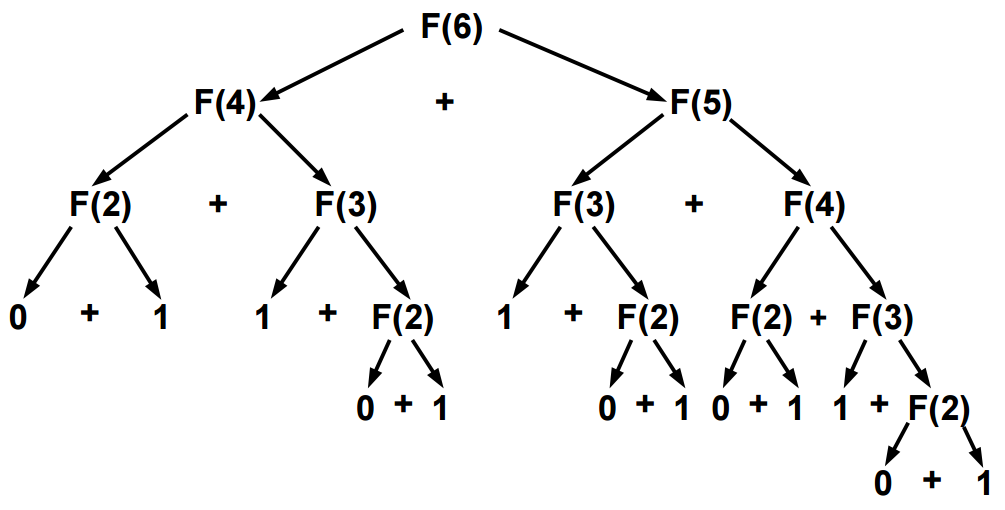
\includegraphics{figs/Aula03/fib_arvore.png}

}

\caption{Árvore de recursão Fib}

\end{figure}

\begin{tcolorbox}[enhanced jigsaw, arc=.35mm, opacityback=0, bottomtitle=1mm, left=2mm, coltitle=black, rightrule=.15mm, colbacktitle=quarto-callout-note-color!10!white, breakable, opacitybacktitle=0.6, bottomrule=.15mm, title=\textcolor{quarto-callout-note-color}{\faInfo}\hspace{0.5em}{Solução}, titlerule=0mm, colframe=quarto-callout-note-color-frame, toprule=.15mm, toptitle=1mm, leftrule=.75mm, colback=white]
\[F(n+2) = F(n+1) + F(n)\]

\[ \begin{bmatrix}F(1) \\ F(2)\end{bmatrix} = \begin{bmatrix}1 \\ 1\end{bmatrix}\]

\[ \begin{bmatrix}F(2) \\ F(3)\end{bmatrix} = \begin{bmatrix}0 & 1 \\1 & 1\end{bmatrix} \begin{bmatrix}F(1) \\ F(2)\end{bmatrix} = \begin{bmatrix}0 & 1 \\1 & 1\end{bmatrix} \begin{bmatrix}1 \\ 1\end{bmatrix}\]

\[ \begin{bmatrix}F(3) \\ F(4)\end{bmatrix} = \begin{bmatrix}0 & 1 \\1 & 1\end{bmatrix} \begin{bmatrix}F(2) \\ F(3)\end{bmatrix} = \begin{bmatrix}0 & 1 \\1 & 1\end{bmatrix}^{2} \begin{bmatrix}1 \\ 1\end{bmatrix}\]

\[ \begin{bmatrix}F(4) \\ F(5)\end{bmatrix} = \begin{bmatrix}0 & 1 \\1 & 1\end{bmatrix} \begin{bmatrix}F(3) \\ F(4)\end{bmatrix} = \begin{bmatrix}0 & 1 \\1 & 1\end{bmatrix}^{3} \begin{bmatrix}1 \\ 1\end{bmatrix}\]

\[\vdots\]

\[ \begin{bmatrix}F(n) \\ F(n+1)\end{bmatrix} = \begin{bmatrix}0 & 1 \\1 & 1\end{bmatrix} \begin{bmatrix}F(2) \\ F(3)\end{bmatrix}= \begin{bmatrix}0 & 1 \\1 & 1\end{bmatrix}^{n-1} \begin{bmatrix}1 \\ 1\end{bmatrix}\]

\begin{itemize}
\item
  considerando \(A = \begin{bmatrix}0 & 1 \\ 1 & 1\end{bmatrix}\), o
  problema se resume a resolver \(A^{n-1}\). Sabemos fazer essa conta?
\item
  Polinômio característico: \(\lambda^2 - \lambda -1=0\)
\item
  Autovalores: \[\lambda_1=\frac{1}{2} + \frac{1}{2}\sqrt{5}\]
  \[\lambda_2=\frac{1}{2} - \frac{1}{2}\sqrt{5}\]
\item
  Autovetores:
\end{itemize}

\[v_1 = \begin{bmatrix}0 & 1 \\1 & 1\end{bmatrix} \begin{bmatrix}x_1 \\ x_2\end{bmatrix} = \lambda_1\begin{bmatrix}x_1 \\ x_2\end{bmatrix}\]

\[v_2 = \begin{bmatrix}0 & 1 \\1 & 1\end{bmatrix} \begin{bmatrix}y_1 \\ y_2\end{bmatrix} = \lambda_2\begin{bmatrix}y_1 \\ y_2\end{bmatrix}\]

\[v_1 = x_1\begin{bmatrix}0 \\ 1\end{bmatrix} + x_2 \begin{bmatrix}1 \\ 1\end{bmatrix} = \left(\frac{1}{2} + \frac{1}{2}\sqrt{5}\right)\begin{bmatrix}x_1 \\ x_2\end{bmatrix}\]

\[v_2 = y_1\begin{bmatrix}0 \\ 1\end{bmatrix} + y_2 \begin{bmatrix}1 \\ 1\end{bmatrix} = \left(\frac{1}{2} - \frac{1}{2}\sqrt{5}\right)\begin{bmatrix}y_1 \\ y_2\end{bmatrix}\]

\begin{itemize}
\tightlist
\item
  resolvendo o sistema acima (pode usar o pacote linag do python para
  calcular os autovalores e autovetores):
\end{itemize}

\[ v_1 = \begin{bmatrix}1, & \frac{1}{2} + \frac{1}{2}\sqrt{5}\end{bmatrix}\]

\[ v_2 = \begin{bmatrix}1, & \frac{1}{2} - \frac{1}{2}\sqrt{5}\end{bmatrix}\]

\begin{itemize}
\tightlist
\item
  Assim, podemos reescrever
\end{itemize}

\[ A^{n-1} = \begin{bmatrix}1 & 1 \\ \frac{1}{2} + \frac{1}{2}\sqrt{5} & \frac{1}{2} - \frac{1}{2}\sqrt{5}\end{bmatrix} \begin{bmatrix}\frac{1}{2} + \frac{1}{2}\sqrt{5} & 0 \\ 0 & \frac{1}{2} - \frac{1}{2}\sqrt{5}\end{bmatrix}^{n-1}\begin{bmatrix}1 & 1 \\ \frac{1}{2} + \frac{1}{2}\sqrt{5} & \frac{1}{2} - \frac{1}{2}\sqrt{5}\end{bmatrix}^{-1}\]

\begin{itemize}
\tightlist
\item
  Sendo assim
\end{itemize}

\[\begin{bmatrix}F(n) \\ F(n+1)\end{bmatrix} = A^{n-1}\begin{bmatrix}1 \\ 1\end{bmatrix}\]
\end{tcolorbox}

\begin{Shaded}
\begin{Highlighting}[]
\ImportTok{import}\NormalTok{ numpy }\ImportTok{as}\NormalTok{ np}
\ImportTok{import}\NormalTok{ math}
\ImportTok{from}\NormalTok{ numpy }\ImportTok{import}\NormalTok{ linalg }\ImportTok{as}\NormalTok{ LA}

\NormalTok{A }\OperatorTok{=}\NormalTok{ np.array([[}\DecValTok{1}\NormalTok{,}\DecValTok{1}\NormalTok{],[}\DecValTok{1}\OperatorTok{/}\DecValTok{2}\OperatorTok{+}\DecValTok{1}\OperatorTok{/}\DecValTok{2}\OperatorTok{*}\NormalTok{math.sqrt(}\DecValTok{5}\NormalTok{), }\DecValTok{1}\OperatorTok{/}\DecValTok{2}\OperatorTok{{-}}\DecValTok{1}\OperatorTok{/}\DecValTok{2}\OperatorTok{*}\NormalTok{math.sqrt(}\DecValTok{5}\NormalTok{)]])}

\NormalTok{L }\OperatorTok{=}\NormalTok{ np.array([[}\DecValTok{1}\OperatorTok{/}\DecValTok{2}\OperatorTok{+}\DecValTok{1}\OperatorTok{/}\DecValTok{2}\OperatorTok{*}\NormalTok{math.sqrt(}\DecValTok{5}\NormalTok{),}\DecValTok{0}\NormalTok{],[}\DecValTok{0}\NormalTok{, }\DecValTok{1}\OperatorTok{/}\DecValTok{2}\OperatorTok{{-}}\DecValTok{1}\OperatorTok{/}\DecValTok{2}\OperatorTok{*}\NormalTok{math.sqrt(}\DecValTok{5}\NormalTok{)]])}
\CommentTok{\#n = int(input("Que termo deseja encontrar: "))}
\NormalTok{n }\OperatorTok{=} \DecValTok{7}
\NormalTok{Fn }\OperatorTok{=}\NormalTok{ A.dot((L}\OperatorTok{**}\NormalTok{(n}\OperatorTok{{-}}\DecValTok{1}\NormalTok{))).dot(LA.inv(A)).dot(np.array([[}\DecValTok{1}\NormalTok{],[}\DecValTok{1}\NormalTok{]]))}

\BuiltInTok{print}\NormalTok{(Fn)}
\end{Highlighting}
\end{Shaded}

\begin{verbatim}
[[13.]
 [21.]]
\end{verbatim}



\end{document}
